感覚運動写像とは,センサー値を変数とする関数によってモーターの出力を決定することであり,
その瞬間のセンサー値だけを使う,最も単純な反応行動のための知能の一つである\cite{asada}.
本研究では,非線形感覚運動写像モデルが使われている.

\subsection{距離データの加重相乗平均}
中央のセンサーによる距離データを $d_{\rm C}$,
また,左のセンサーによる距離データを $d_{\rm L}$ とする.
それらを用いて,左の感覚運動写像の入力 $x_{\rm L}$ を加重相乗平均によって
求める(式(\ref{eq:xL})).
同じように,$d_{\rm C}$と右のセンサーから得られた距離データ $d_{\rm R}$を
用て右の感覚運動写像の入力 $x_{\rm R}$ を求める(式(\ref{eq:xR})).
\begin{eqnarray}
  %x_{\rm L} &=& e^{\gamma \ln d_{\rm C}} \cdot e^{(1-\gamma)\ln d_{\rm L}} 
  x_{\rm L} &=& d_{\rm C}^{\gamma} \times d_{\rm L}^{(1-\gamma)}
  \label{eq:xL} \\
  %x_{\rm R} &=& e^{\gamma \ln d_{\rm C}} \cdot e^{(1-\gamma)\ln d_{\rm R}} 
  x_{\rm R} &=& d_{\rm C}^{\gamma} \times d_{\rm R}^{(1-\gamma)}
  \label{eq:xR}
\end{eqnarray}
$\gamma$は重みであり,本研究においては$\gamma=0.33$とする.
$\gamma=\frac{1}{3}$とすることにより,左のセンサー,中央のセンサーおよび右の
センサーがそれぞれ,$\frac{2}{3}$の等加重となる.

\subsection{感覚運動写像}
式(\ref{eq:xL})と式(\ref{eq:xR})で得られた$x_{\rm L}$と$x_{\rm R}$を式(\ref{eq:mR})と
式(\ref{eq:mL})に代入して,ロボットの右モーターの出力($m_{\rm R}$)と左モーターの
出力($m_{\rm L}$)を計算する.
係数$\alpha$がロボットの最大速度を制御する,係数$\beta$が{\rm tanh}の傾きを制御する.
係数$b$が関数の変曲点の位置を制御する,係数$c$が関数の縦軸上の位置を制御する.
\begin{eqnarray}
\begin{aligned}
  m_{\rm R} = &\alpha \tanh(\beta_1(x_{\rm L} - b_{\rm L})) + \\
        &\alpha \tanh(\beta_2(x_{\rm L} - b_{\rm L})) + c
 \label{eq:mR}
\end{aligned}
\end{eqnarray}

\begin{eqnarray}
\begin{aligned}
  m_{\rm L} = &\alpha \tanh(\beta_1(x_{\rm R} - b_{\rm R})) + \\
        &\alpha \tanh(\beta_2(x_{\rm R} - b_{\rm R})) + c
 \label{eq:mL}
\end{aligned}
\end{eqnarray}
 
今回の実験のパラメーターは
$\alpha=30\%$とする.
すなわちロボットは最高速度の60\%の速度で走行する.
$\beta_1=0.004$,
$\beta_2=10$,
$c=0$とする.
ロボットグループ1の$b_{\rm L}$とロボットグループ2の$b_{\rm R}$は160mm,
また,ロボットグループ2の$b_{\rm L}$とロボットグループ1の$b_{\rm R}$は260mmである.

\subsection{パラメーター$b$の説明}
$b_{\rm L}=260$mm(図\ref{fitan}のB点),$b_{\rm R}=160$mm(図\ref{fitan}のA点)の場合,
$b_{\rm L}=260$mmのtanh関数の変曲点が$b_{\rm L}=160$mmのtanh関数の変曲点より横軸の正方向に
100移動する(図\ref{fitan}の$B$点).左右の距離データ($d_{\rm L}$と$d_{\rm R}$)が同じでも($x_{\rm L}$と$x_{\rm R}$も同じ)
式(\ref{eq:mR})の$x-b_{\rm L}$が式(\ref{eq:mL})の$x-b_{\rm R}$より小さくなるので,
右のモーター(($m_{\rm R}$))が左のモーター(($m_{\rm L}$))より小さくなり,右のモーターが遅いので,ロボットが右曲がりやすいと認定する.
左に曲がり易いのは,逆の設定である.
%\vspace{-9mm}
\begin{figure}[!ht]
    \centering
    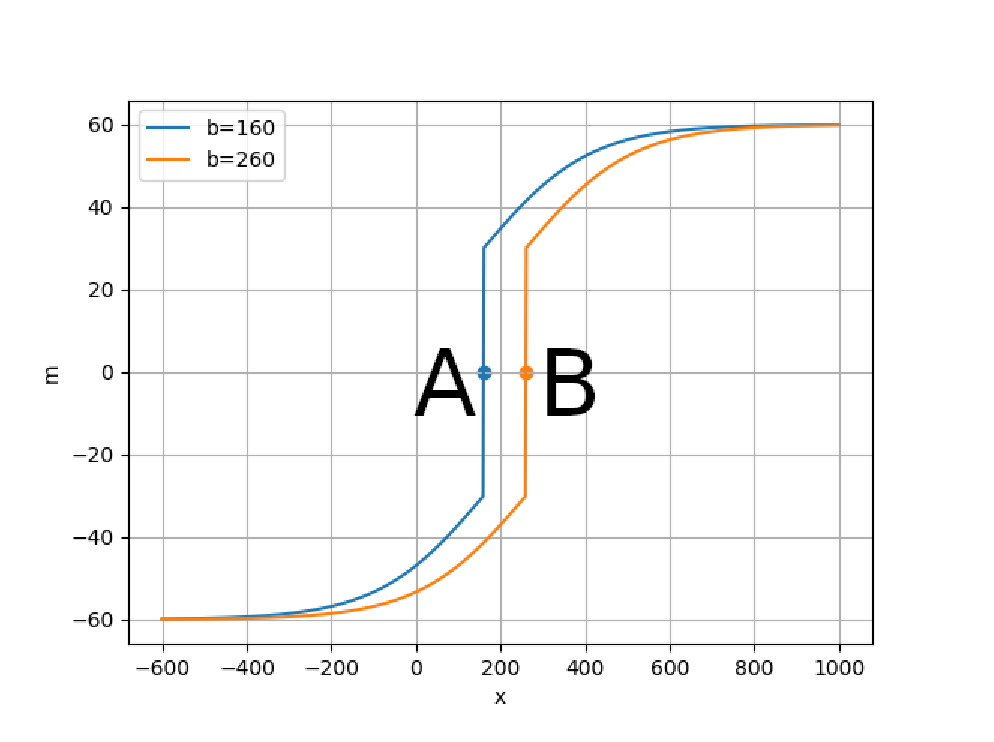
\includegraphics[width=0.7\linewidth]{tanh.eps} 
    \caption{$b=160$mmと$b=260$mmのtanh関数の曲線}
    \label{fitan}
\end{figure}

